Overall, the proposed system has been reduced to the functional blocks shown in Figure \ref{systemBD} below. On the input side of the system, the two stereo cameras are physically connected to two video memory buffers, and the camera controls and video memory buffer data are accessed through programmable logic on the Zynq processor.  Since the rangefinder and IMU modules each communicate with UART and SPI interfaces, respectively, each are connected directly to the Zynq's dual-core ARM processor. Both sensors may then be communicated with using Xilinx's built-in ARM peripheral drivers, reducing overall implementation time. Note that an I$^2$C controller is also included as a peripheral for the ARM processor, allowing for communication with each camera's control registers. 
\par
\begin{figure}[H] 
	\centerline{
	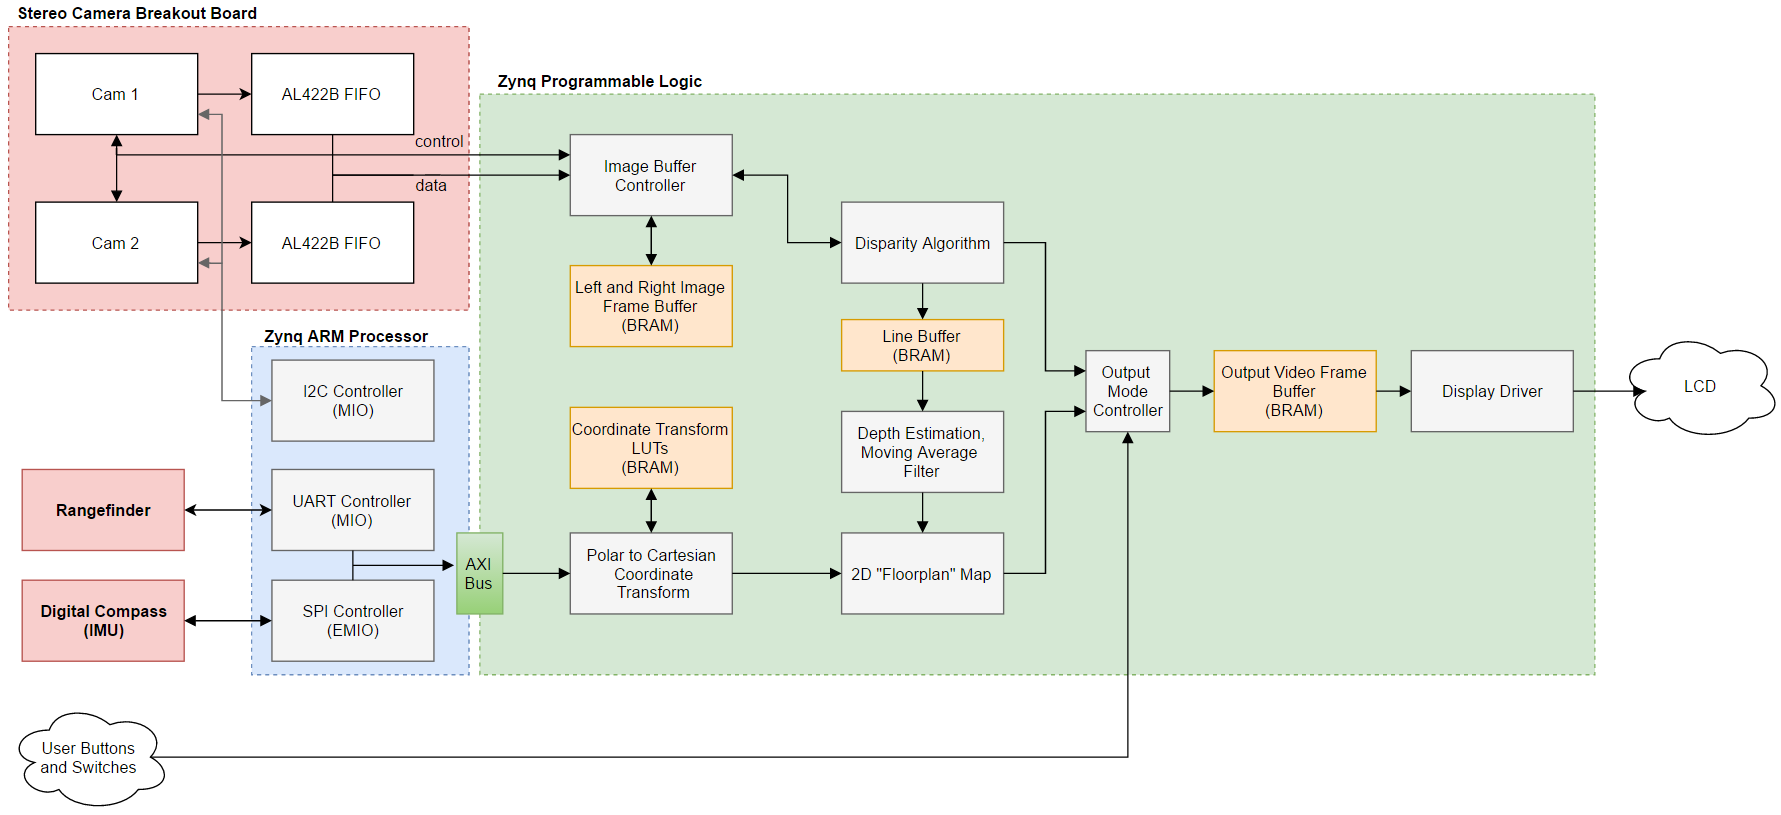
\includegraphics[width=1.25\linewidth]{full_blockdiag.png}
	}
	\caption{System Block Diagram}
	\label{systemBD}
\end{figure}
\par
In terms of stereo camera data processing, the first stage of programmable logic consists of a dual image buffer controller used for triggering image captures and reading image data into local memory on the ZedBoard. A disparity module then reads in image data from local memory, and calculates the relative offset between objects contained in the stereo image pair. A portion of this data is then stored in local memory for correlation with data from the 2D scanning laser rangefinder. Depending on the position of the ZedBoard's user input switches, the output from the disparity algorithm is also passed to a video frame buffer and displayed via VGA. 
\par
In order to correlate disparity data with the 2D depth information from the scanning laser rangefinder, several horizontal lines of pixel data from the disparity algorithm are averaged together. This single line of depth information can be compared to the single line of depth information from the rangefinder. However, due to differences in the field of view of each sensor, the depth information is passed through a moving average filter before being correlated with rangefinder data. 
\par
Data from the scanning laser rangefinder and IMU modules is pre-processed in programmable software, allowing for the estimation of sensor rotation relative to the IMU's compass heading.  A custom AXI peripheral bus is then used to pass data from the programmable software to the programmable hardware. At this stage, a pair of lookup tables are used to convert the rangefinder data from Polar to Cartesian coordinates, and the modified data is correlated with depth estimation data from the disparity algorithm. Depending on the status of the ZedBoard's user switches, the 2D floorplan map created using the combined sensor data is then passed to the output video buffer for external display. 